Ergebnis der experimentellen Hybrid-Cloud Aufstellung ist ein speziell konfigurierter Spectrum Scale Speichercluster mit Anbindungen an den \ac{COS} und eine neu entwickeltet Cloudanwendung mit Verbindung zu dem Objektspeicher und einem exemplarischen Analysedienst für Imagedateien.
Das aktuelle Setup ist ein VM-Abbild, das auch auf einer einzelnen Maschinen für Demozwecke verwendet werden kann.

Der Austausch von Daten zwischen Cluster und Cloud finden problemlos statt. Es muss nur darauf geachtet werden, dass keine Verschlüsselung beim Sharing stattfindet.

Einzige Schwierigkeit ist die Aktualisierung der Dateiliste auf der Seite von Spectrum Scale, da keine Funktion hierfür vorgesehen ist. Zur Lösung dieses Problems wird eine, alle vom Cluster exportieren Dateien enthaltende, Manifestdatei von Scale angelegt und in den Cloudspeicher hochgeladen. Die Demoanwendung kann nun diese Liste selber aktualisieren. Beim Importieren beginnt Scale mit dieser Manifestdatei und kann, anhand von ihr, alle anderen neuen Dateien herunterladen.

Die Demo stellt eine graphische Schnittstelle zum Speichern, Ansehen und Analysieren von Bilddateien und ist über IBM Bluemix erreichbar. Sie wird von einem express Server präsentiert, der ebenfalls eine einfache REST-API zum verwenden der oben beschriebenen Funktionen bereitstellt. Für die Bildanalyse wird IBM Watson Image Recognition verwendet, ein Dienst der mithilfe von Deep Learning Bilder klassifizieren kann.

Insgesamt funktioniert der Aufbau sehr gut und eine hohe Performanz wird bei einzelnen Anfragen geliefert, sodass sich das Szenario ausgezeichnet für Demozwecke verwendet werden kann.

\textbf{Verifikation der Anwendung}

In \autoref{fig:demooverviewlist} sieht man die Startseite der Anwendung. Hier sieht man eine Liste aller hochgeladenen Dateien in \ac{COS} zusammen mit Informationen über Dateigröße, Veränderungsdatum und Dateipfad. Jede Datei kann betrachtet werden oder, falls es sich um ein Bild handelt, klassifiziert werden. 

\begin{figure}[hbt]
	\centering
	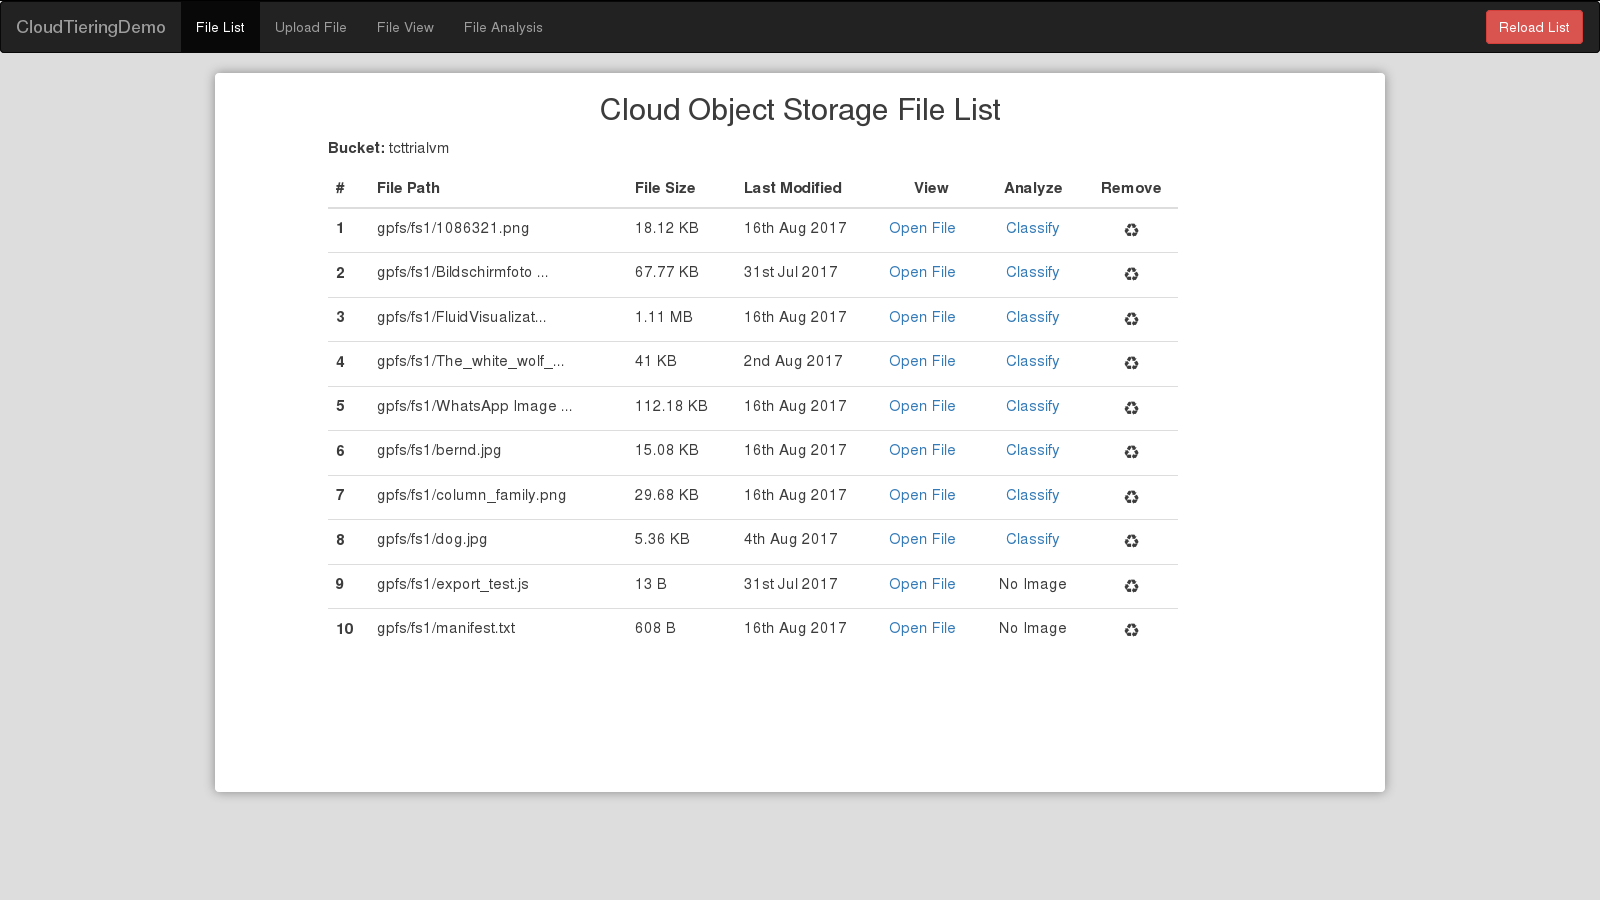
\includegraphics[scale=0.25]{images/demo-overview-list}
	\caption{Liste aller COS-Dateien in der Demo}
	\label{fig:demooverviewlist}
\end{figure}

\begin{figure}[hbt]
	\centering
	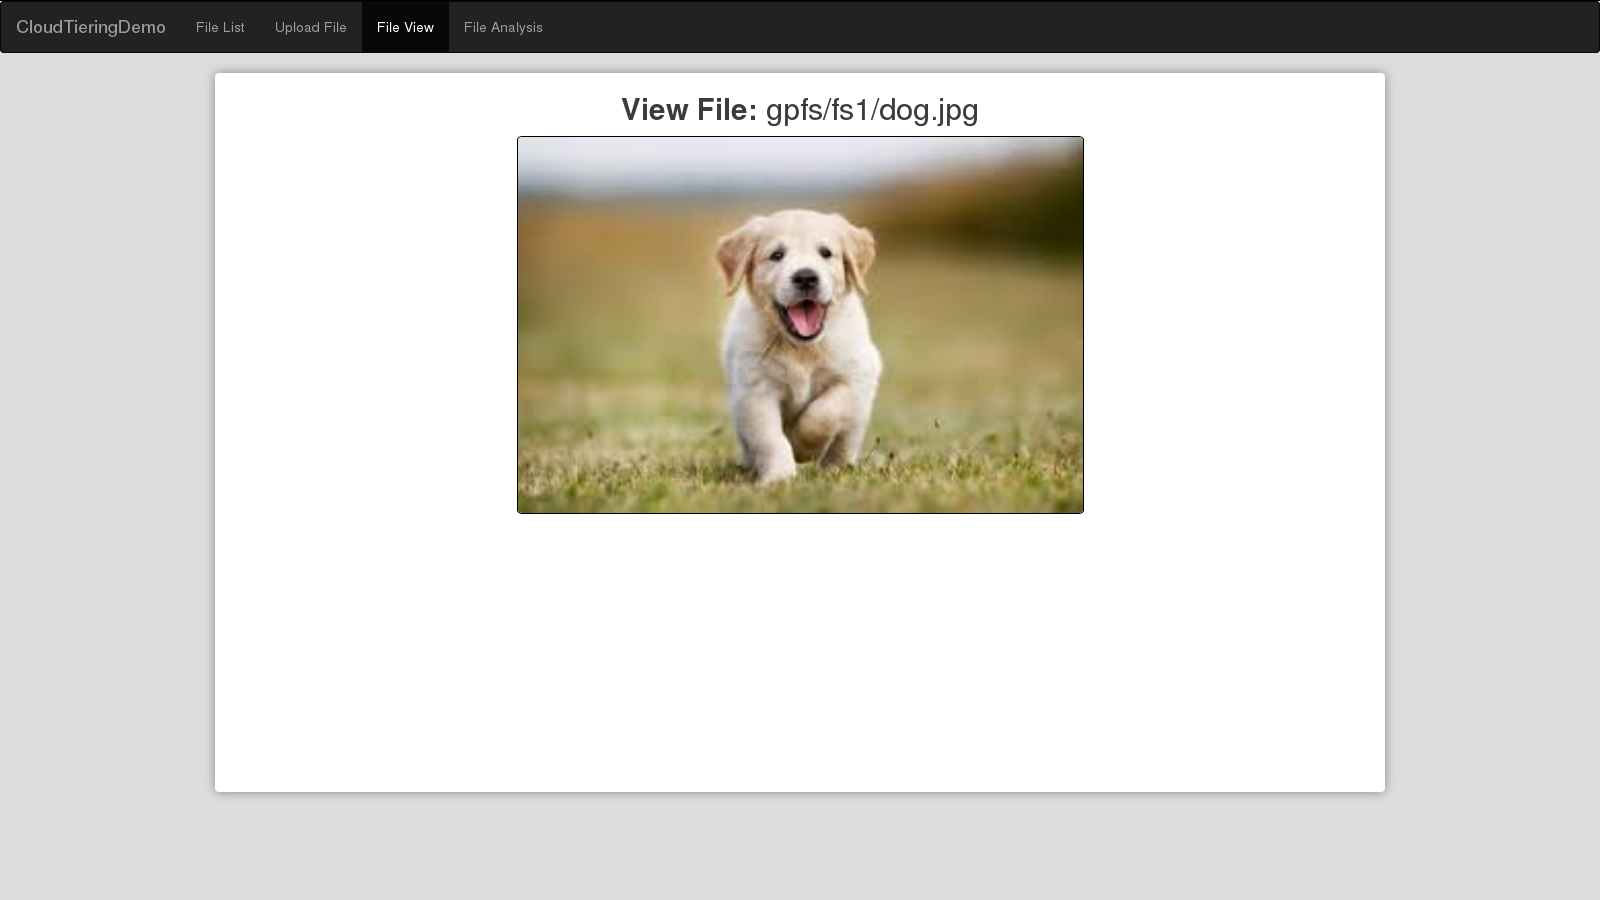
\includegraphics[scale=0.25]{images/demo-overview-view}
	\caption{Ansicht einer COS-Dateien in der Demo}
	\label{fig:demooverviewview}
\end{figure}

Je nach zu betrachtender Datei wird eine unterschiedliche Ansicht, beim Aktivieren des Links zum Öffnen, aktiviert. Bilder werden skaliert und angezeigt (siehe \autoref{fig:demooverviewview}), Texte in ein Feld eingebettet und alle anderen Formate zum Download angeboten.

Wird von der Startseite die Klassifizierung eines Bildes ausgewählt sieht man \autoref{fig:demooverviewanalysis}. In einer Liste werden die einzelnen erkannten Merkmale mit ihrer jeweiligen Verlässlichkeit angezeigt. Oberhalb von dieser befindet sich ein Link zur Dateiansicht.
\begin{figure}[hbt]
	\centering
	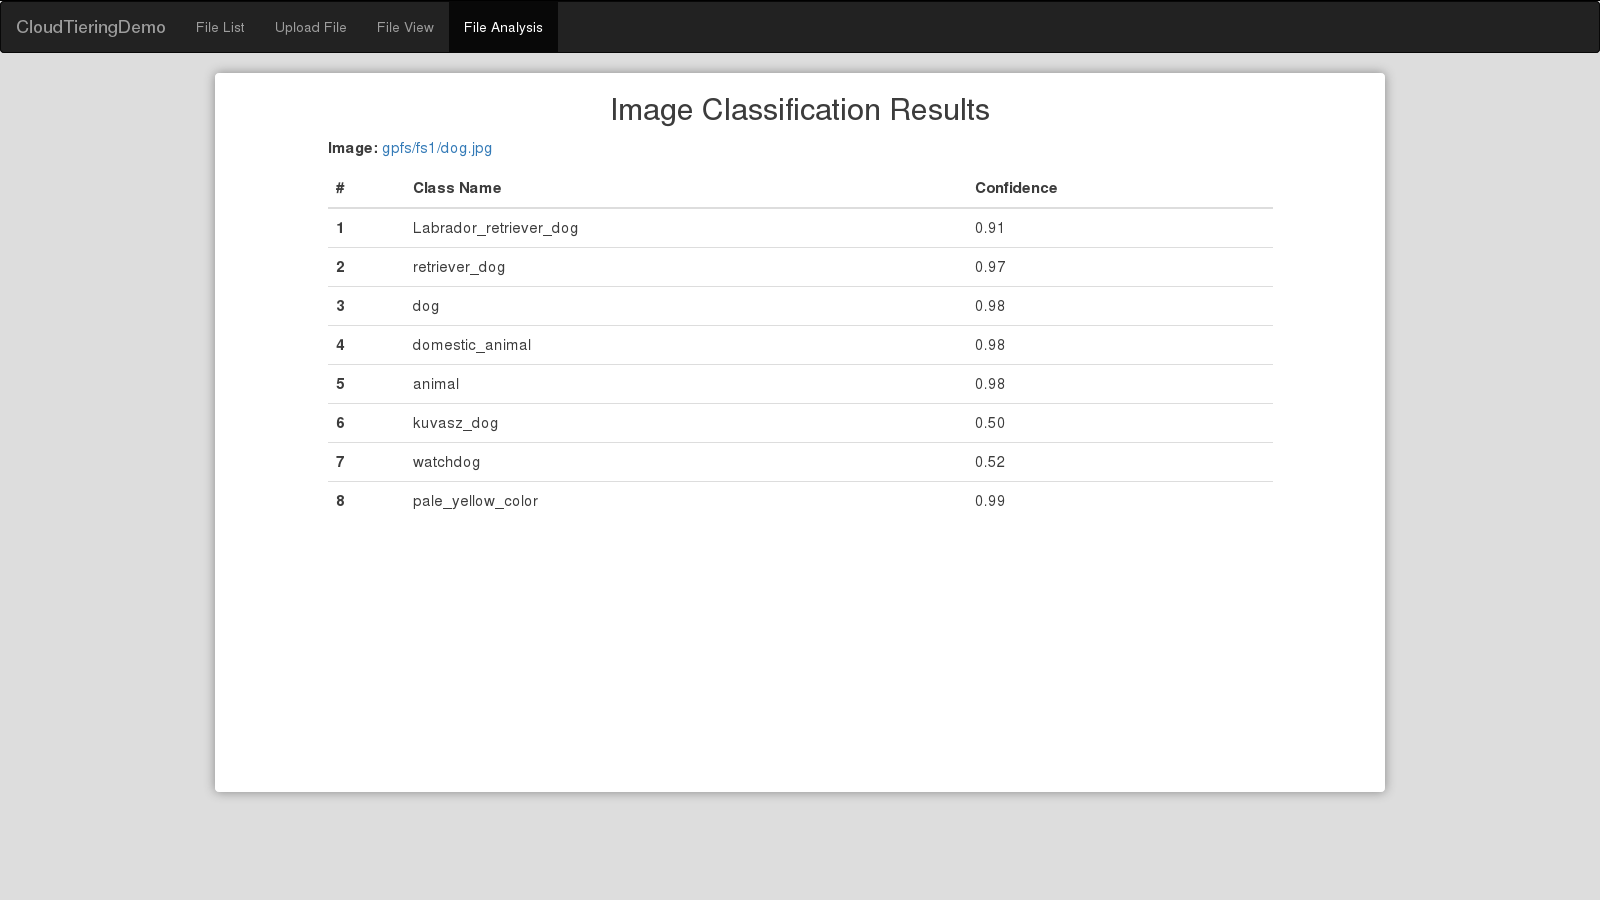
\includegraphics[scale=0.25]{images/demo-overview-analysis}
	\caption{Analyseergebnisse einer COS-Dateien in der Demo}
	\label{fig:demooverviewanalysis}
\end{figure}

Ebenfalls können neue Dateien über die Web-UI (siehe \autoref{fig:demooverviewupload}) hochgeladen werden. Nach Auswahl im Filesystem des Nutzers und nachfolgendem Upload wird eine kurze Bestätigung per Toast wiedergegeben.
\begin{figure}[hbt]
	\centering
	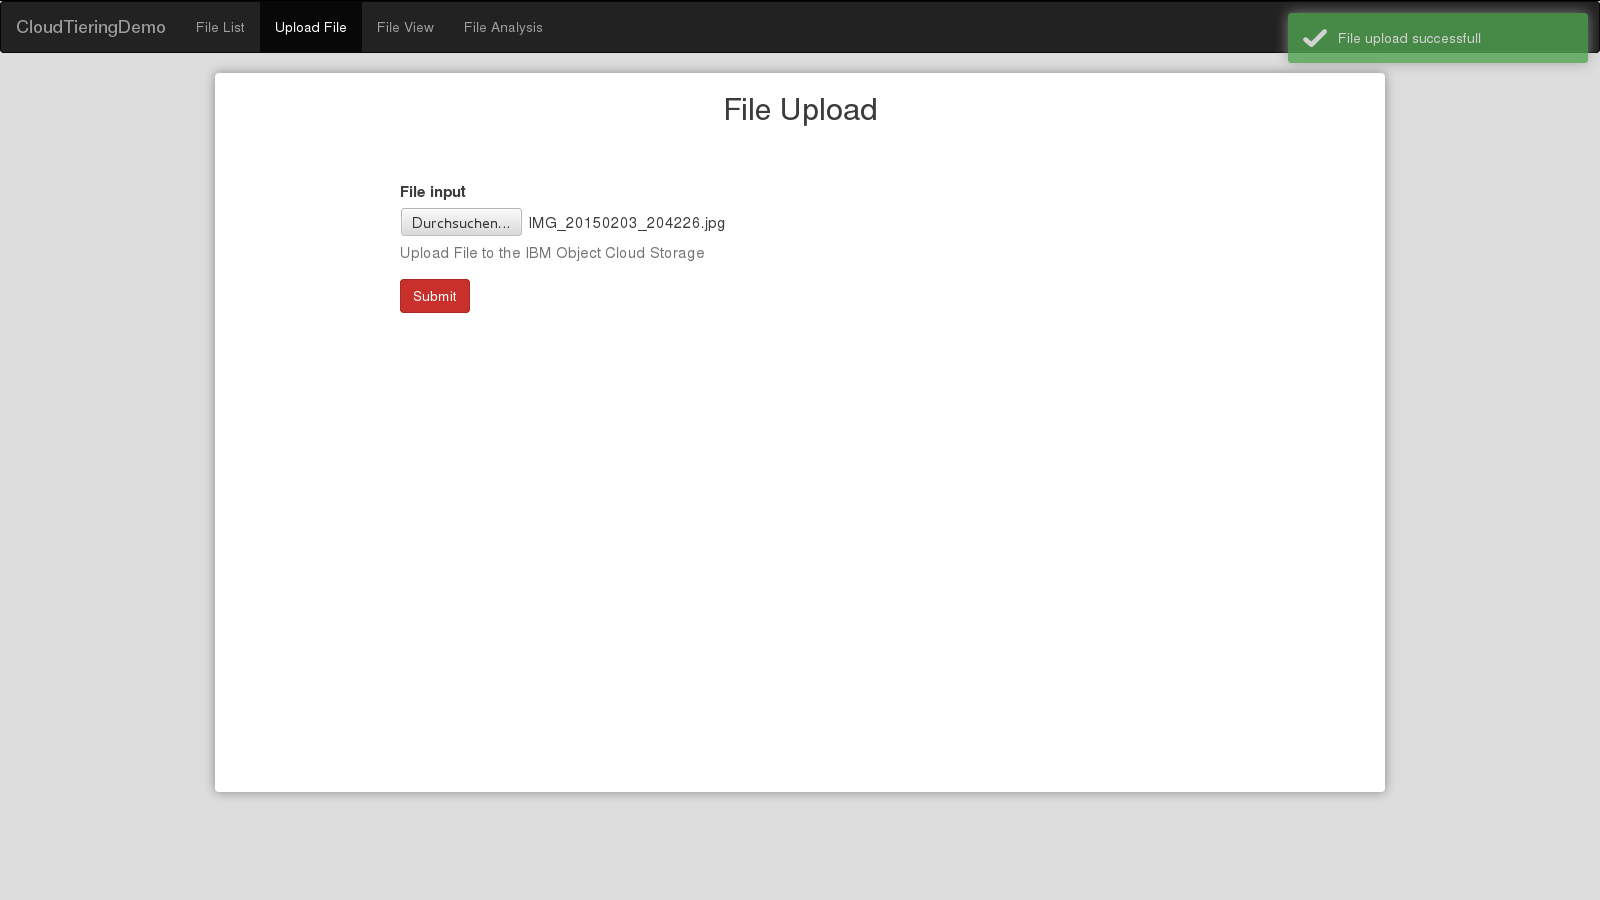
\includegraphics[scale=0.25]{images/demo-overview-upload}
	\caption{Upload einer neuen Datei zu COS in der Demo}
	\label{fig:demooverviewupload}
\end{figure}